\chapter{Описание предлагаемого подхода}
\label{chapter2}

Задача данной главы - описание задачи Needle, подходов к её решению, а так же уже полученные временные оценки, основанные на принципе минимакса. Важной частью данной главы является описание применения к задаче black-box подхода.

\section{Рассматриваемая оптимизационная задача}

Прежде чем описывать задачу, введем некоторые вспомогательные утверждения:

\begin{prop}[Принцип минимакса Яо\cite{5}]
Если задача состоит из конечного набора экземпляров фиксированного размера и допускает конечное множество детерминированных алгоритмов, тогда матожидание времени работы рандомизированного алгоритма не меньше, чем среднее (по экземплярам задачи) время работы лучшего детерминированного алгоритма.
\end{prop}


\begin{prop}
Если black-box задача определена на пространстве поиска $S$, сложность black-box сложность ограничена сверху $ \frac{(| S | + 1)}{2}$ \cite{2}.
\end{prop}



\begin{proof}
    Мы создаем равномерно случайную перестановку S и запрашиваем точки поиска в этом случайном порядке. Для каждого $s \in S$ время ожидания запроса равно  $ \frac{(| S | + 1)}{2}$.
\end{proof}


\subsection{Задача Needle}
Рассматриваемая в работе задача в области оптимизационных алгоритмов известна как Needle, или <<иголка в стоге сена>>. Формально задача сформулирована следующим образом: 

Для всех $z \in \{0, 1\}^n \;\;\; $  
    \begin{math} 
    f_{z} : \{0, 1 \}^n \rightarrow \{0,1\}; x \rightarrow  \left\{ \begin{array}{ll}
    1 & \textrm{$x = z$}\\
    0 & \textrm{$x \ne z$}
    \end{array} \right.
    \end{math}

Needle является одной из сложных задач, так как за каждый запрос алгоритм получает лишь знание, совпадает ли запрос с оптимумом или нет, и никаких выводов о других запросах сделать не может. 

\begin{myth}
Black-box сложность задачи Needle равна $\frac{2^n + 1}{2}$.
\end{myth}
\begin{proof}
    Вехняя оценка сложности следует из Утверждения 4. Нижнюю оценку можно получить из принципа минимакса Яо, прописанного в Утверждении 3.
    Мы считаем равномерное распределение на всей $N_a$, где $a \in S$. После того, как будут запрошены m точек множества без определения оптимума задачи, все остальные $|S| - m$
    точек имеют ту же вероятность быть оптимумом. Следовательно, каждая детерминированная стратегия поиска запросов равняется $\frac{2^n + 1}{2}$ различных точек пространства поиска.
\end{proof}

Так как за каждый запрос алгоритм получает лишь знание, совпадает ли запрос с оптимумом или нет, то никаких выводов о других запросах он сделать не может, и единственное, что он может сделать~--- не 
запрашивать уже запрошенное повторно. Таким образом, лучший детерминированный алгоритм просто делает все возможные запросы по порядку, и среднее число запросов до оптимума - ровно $\frac{2^n + 1}{2}$

Такое же время работы у алгоритма, который генерирует случайную перестановку чисел от 0 до $(2^n - 1)$ и спрашивает их в этом порядке. Верхняя и нижняя оценка совпадают.

Так как решение задачи Needle в рамках black-box сложности не зависят от самой задачи, то найденные идеи решения задачи могут помочь в будущем в исследовании других задач, в частности,
оценить время обхода плато~\cite{6}, достаточно часто встречающееся в оптимизационных задачах. 

\subsection{Описание подхода}

Будем рассматривать классы алгоритмов для операторов на несмещенных сложностях. Решения, принимаемые алгоритмом, могут зависеть только от наблюдаемых значений функции, но не от самих точек. 
Также алгоритм может делать запросы, полученные только при помощи несмещенных операторов, обладающих двумя свойствами: инвариантностью относительно перестановки и инвариантностью относительно 
побитового исключающего или. 
	
Наибольший интерес представляют собой алгоритмы для операторов  несмещенных сложностей арности $k = 1, 2, 3$.

Время работы black-box алгоритма оценивается числом запросов к черному ящику,  то есть это ожидаемое число запросов до точки  нахождения оптимума.
	
Подсчет верхних оценок сводится к разработке алгоритма и оценке времени его работы.
	
Подсчет нижних оценок сводится к нахождению общего вида всех алгоритмов данного класса, нахождению параметров, однозначное определяющих работу алгоритма, построению выражения, 
зависящего от указанных параметров и определяющего математическое ожидание времени работы алгоритма, и минимизации времени работы.  

\subsection{Black-box оптимизация задачи Needle}

Needle является достаточно простой в обычном случае, но при этом достаточно сложна в black-box модификации.

Задача представляется оптимизирующему алгоритму, представленному в виде черного ящика, к которому можно задавать запросы, и он возвращает либо 1, если запрос совпал с загаданной строкой, 
либо 0 в обратном случае. 

\begin{figure}[H]
\caption{}\label{fig3}
    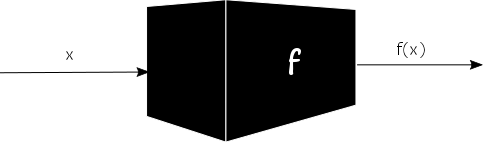
\includegraphics[height=5cm]{pic/blackbox.png}
\end{figure}

Запросы к черному ящику можно генерировать либо случайным образом, либо основываясь на результаты предыдущих запросов. В лучшем случае, алгоритм может не запрашивать уже запрошенное повторно.

\chapterconclusion

В данной главе была поставлена решаемая задача, а так же ожидаемые к ней подходы в модели несмещенной blaсk-box сложности. Также были описаны уже существующие решения и оценки их работы, что 
демонстрирует научную новизну представленной работы. 
